\documentclass[a4paper,twocolumn,11pt]{article}
\usepackage{graphicx}
\usepackage{flushend}
\usepackage{url}
\usepackage{natbib}
\usepackage[T1]{fontenc}
\usepackage{helvet}
\renewcommand{\familydefault}{\sfdefault}
\usepackage[utf8]{inputenc}
\usepackage[spanish,es-tabla]{babel}
\parindent=0.7cm
\hbadness=10000
\vbadness=10000
\usepackage{amsmath,amssymb,amsfonts,latexsym,cancel}
\usepackage{array,bm,float,fancyhdr,graphicx,multirow,subfig,geometry}
\usepackage[table]{xcolor}
\usepackage{tikz}
\usetikzlibrary{arrows.meta,positioning}
\usepackage{comment,booktabs,hyperref,pifont,titlesec,authblk}
\raggedbottom
\graphicspath{{../figures/}}
\newcommand{\grad}{$^{\circ}$ }
\geometry{lmargin=2cm,rmargin=2cm,top=2.5cm,headsep=0.5cm,headheight=1.65cm,bottom=2cm}
\titleformat*{\section}{\small\bfseries\sffamily}
\titleformat*{\subsection}{\small\bfseries\sffamily}
\titleformat*{\subsubsection}{\small\bfseries\sffamily}
\titleformat*{\paragraph}{\small\bfseries\sffamily}
\titlespacing*{\section}{0pt}{0.6ex}{0.4ex}
\titlespacing*{\subsection}{0pt}{0.5ex}{0.3ex}
\pagestyle{fancy}
\lhead{}\chead{\includegraphics[height=1.5cm]{JJII_logo.png}}\rhead{}\lfoot{}\rfoot{}
\fancypagestyle{firststyle}{\fancyhf{}\fancyfoot[C]{\footnotesize \thepage}\fancyhead[C]{\includegraphics[height=1.5cm]{JJII_logo.png}}}
\renewcommand{\headrulewidth}{1.5pt}
\usepackage[normalem]{ulem}
\usepackage[labelfont=bf,hypcap=false]{caption}
\usepackage{stfloats}
\setlength{\affilsep}{0.2em}
\renewcommand\Authsep{\\}\renewcommand\Authand{\\}\renewcommand\Authands{\\}

\begin{document}
\title{\textbf{Ingeniería y Tecnología\\ Desarrollo de un Prototipo de Procesamiento Local para la Detección, Clasificación y Análisis Predictivo de Manchas Solares mediante Visión Computacional e Inteligencia Artificial}}
\author[1]{\small Autor: Benítez, Carlos}
\author[1,2]{\small Orientadores: Cabral, Juan; Stalder, Diego; Gómez, José María; Schaerer, Christian; Núñez, Jesús}
\affil[1]{Facultad de Ingeniería, Universidad Nacional de Asunción}
\affil[2]{Facultad Politécnica, Universidad Nacional de Asunción}
\date{}

\twocolumn[
\begin{@twocolumnfalse}
\maketitle
\section*{Resumen}
El presente trabajo desarrolla un prototipo funcional para la detección, clasificación y análisis predictivo local de manchas solares mediante visión computacional e inteligencia artificial. El sistema integra una cadena de procesamiento que vincula captura heliográfica en luz blanca, registro de metadatos, sincronización con base de datos, inferencia local y visualización web. La cadena de procesamiento incorpora YOLO26n para el agrupamiento de regiones activas, un modelo jerárquico basado en ConvNeXtV2a para clasificación Zurich--McIntosh que preserva dependencias semánticas entre $Z$, $P$ y $C$, y módulos predictivos complementarios para el número de manchas solares mediante un filtro PVL--Kalman y para la distribución latitudinal de la actividad mediante Descomposición en Modos Dinámicos aplicada al diagrama de Spörer. El prototipo fue validado mediante métricas experimentales sobre un conjunto de datos construido a partir de imágenes SDO/HMI, reportes NOAA SRS y registros propios, además de pruebas de operación embebida, inferencia ONNX y consistencia taxonómica. Los resultados muestran que la arquitectura propuesta permite observaciones solares trazables, portables e interpretables en observatorios académicos locales \citep{ultralyticsYOLO26,woo2023convnextv2,raspberryPi5Docs2026}.

\textbf{Palabras clave:} manchas solares, visión computacional, inteligencia artificial, Zurich--McIntosh, PVL--Kalman, DMD, YOLO26n, ConvNeXtV2a, Raspberry Pi 5.
\vspace{0.1cm}
\end{@twocolumnfalse}
]
\thispagestyle{firststyle}

\section{Introducción}
El análisis automático de manchas solares constituye un punto de partida en la física solar, ya que sienta las bases para el monitoreo operativo de la actividad fotosférica y para la prevención de eventos capaces de afectar sistemas electrónicos y de comunicación. Las regiones activas concentran campos magnéticos intensos y se manifiestan como estructuras oscuras en observaciones de luz blanca. En observatorios terrestres y académicos persiste un problema operativo: la adquisición de imágenes, el registro de metadatos, la identificación de grupos y la clasificación morfológica suelen ejecutarse como tareas separadas, con alta dependencia de revisión manual. Por ello, la trazabilidad entre captura original, condiciones instrumentales, recortes derivados y clasificación posterior resulta limitada \citep{hathaway2015solarcycle,mcintosh1990classification,noaaSRS,usaf2003sunspot}.

Este trabajo presenta una cadena operativa completa de adquisición, procesamiento local, clasificación y análisis predictivo. El prototipo combina cámara monocromática ZWO ASI174MM Mini, cuña de Herschel, telescopio refractor Vixen de $D=60$ mm y $F=420$ mm, Raspberry Pi 5, base de datos Supabase y una plataforma web con inferencia ONNX. A diferencia de una solución centrada solo en entrenamiento de modelos, la propuesta articula instrumentación, software, persistencia de datos y soporte interpretativo: cada observación puede ubicarse dentro de la tendencia temporal del ciclo solar y contrastarse con patrones esperados de actividad. La arquitectura busca portabilidad para observatorios académicos con recursos computacionales y conectividad variables \citep{zwoASI174Manual2025,luntWhiteLightWedges2026,raspberryPi5Docs2026,camporeale2019ml,clette2014revisiting}.

\section{Objetivos}
\subsection{Objetivo general}
Desarrollar un prototipo funcional para la detección y clasificación local de manchas solares, integrando técnicas de visión por computadora, inteligencia artificial y análisis predictivo de actividad solar para observatorios locales.
\subsection{Objetivos específicos}
\begin{itemize}
    \item Analizar registros históricos de manchas solares a partir de imágenes heliográficas y datos astronómicos.
    \item Diseñar un flujo de adquisición y preprocesamiento de imágenes para vincular observaciones solares con reportes internacionales.
    \item Desarrollar un detector YOLO26n para localizar grupos solares y un clasificador jerárquico ConvNeXtV2a para inferir caracteres Zurich--McIntosh preservando dependencias semánticas.
    \item Implementar un módulo predictivo para la evolución temporal del índice de manchas solares y la distribución latitudinal de la actividad.
    \item Integrar el sistema en una arquitectura híbrida con plataforma web, base de datos e inferencia local.
    \item Validar el sistema mediante métricas de detección, clasificación, coherencia predictiva, operación embebida y consistencia física.
\end{itemize}

\section{Materiales y métodos}
\subsection{Arquitectura general del sistema}
La arquitectura propuesta integra adquisición local, preprocesamiento, almacenamiento, inferencia y visualización. La separación modular permite actualizar el hardware de captura, los modelos de inferencia o la capa de visualización sin romper la trazabilidad entre imagen original, metadatos, recortes, etiquetas y productos predictivos. El flujo se organiza como una cascada: primero se registra la observación y sus condiciones, luego se normaliza la imagen de disco completo, se detectan grupos solares, se generan recortes normalizados y finalmente se calculan probabilidades morfológicas y productos predictivos consultables desde la plataforma web.

\subsection{Hardware de observación y procesamiento}
\begin{figure*}[p]
    \centering
    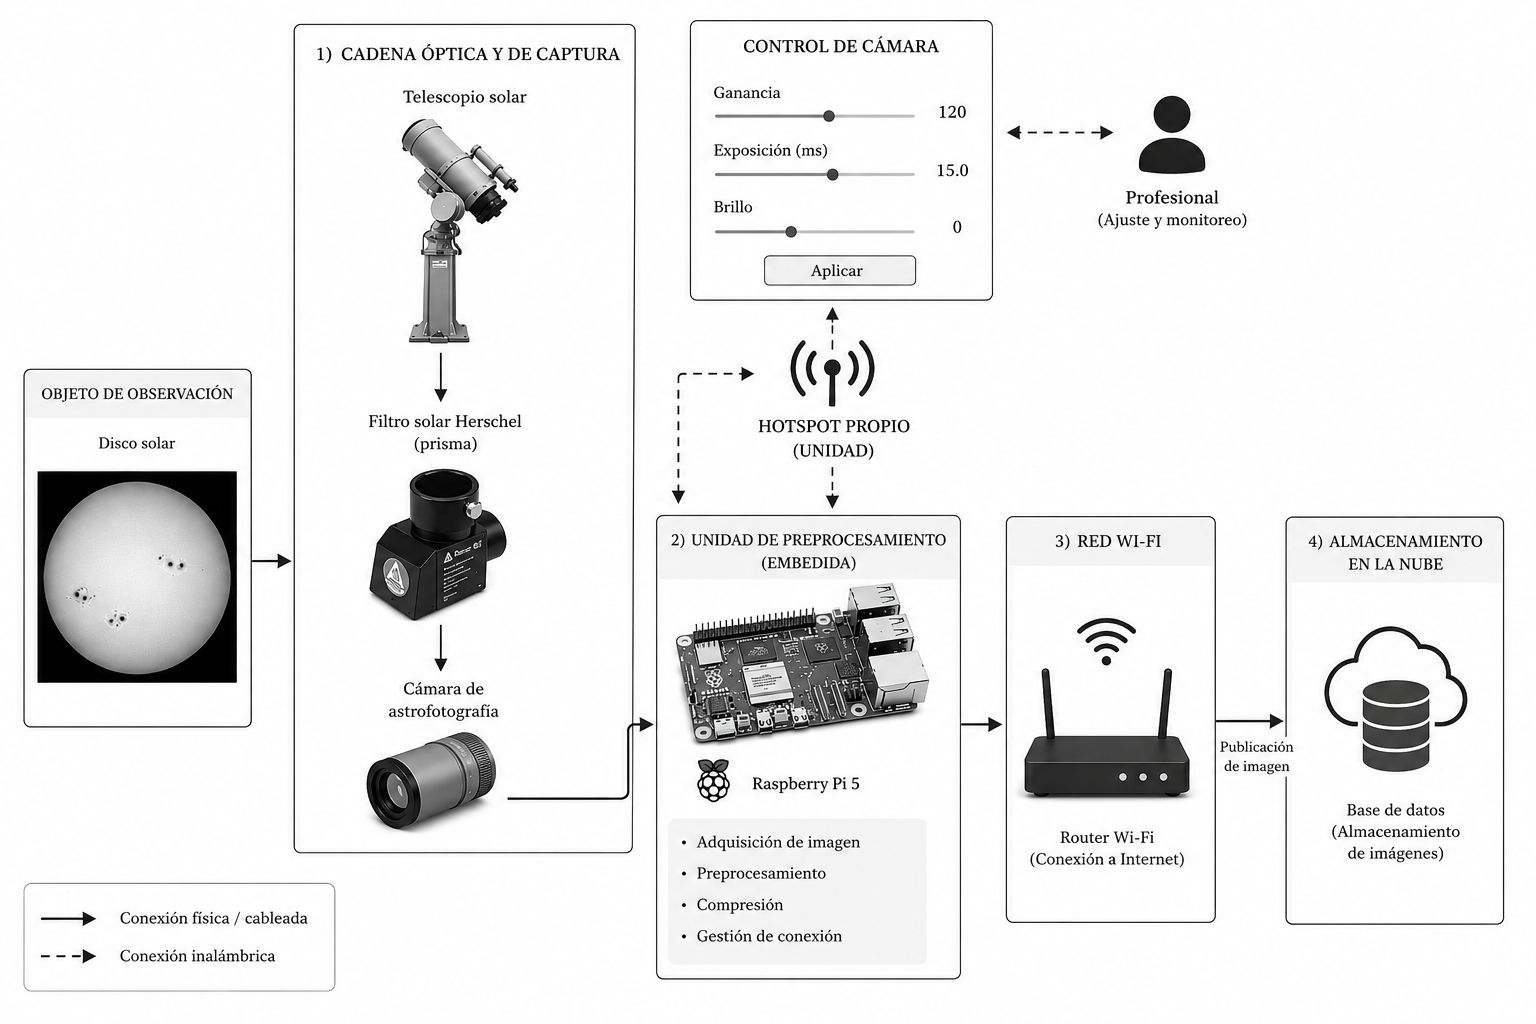
\includegraphics[height=0.42\textheight,keepaspectratio]{hw/module.png}
    \caption{Módulo de observación solar implementado.}
    \label{fig:modulo-observacion}
\end{figure*}
\begin{figure*}[p]
    \centering
    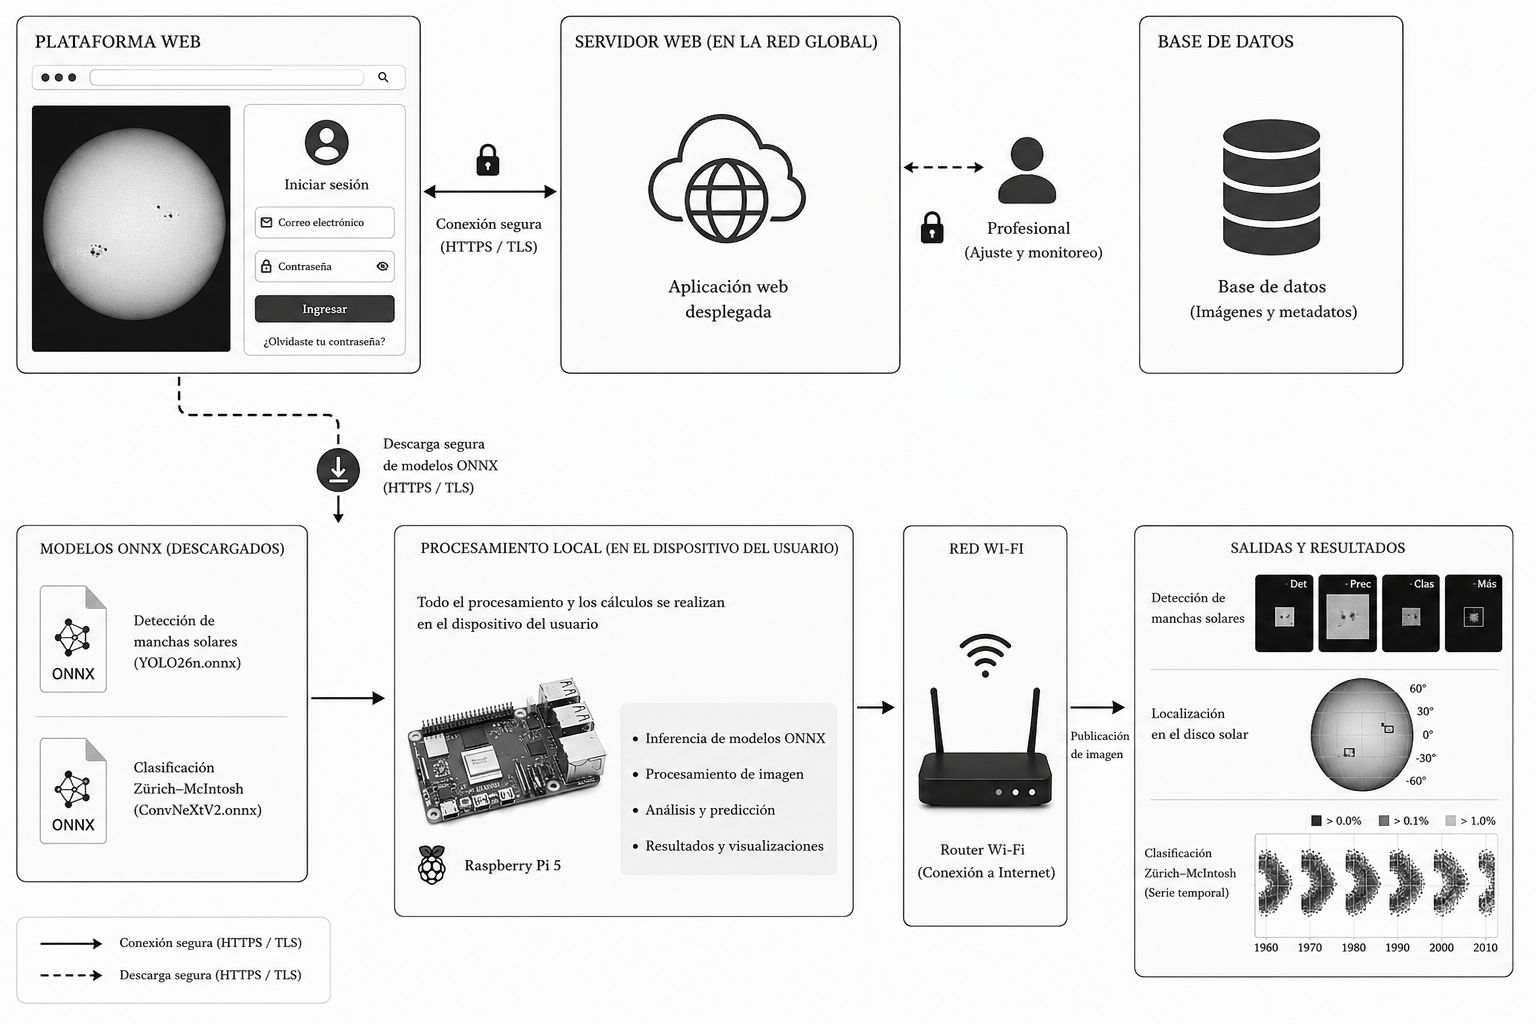
\includegraphics[height=0.42\textheight,keepaspectratio]{hw/camera_mount.png}
    \caption{Montaje de cámara y filtro para captura solar en luz blanca.}
    \label{fig:montaje-camara-filtro}
\end{figure*}
\begin{figure*}[t]
    \centering
    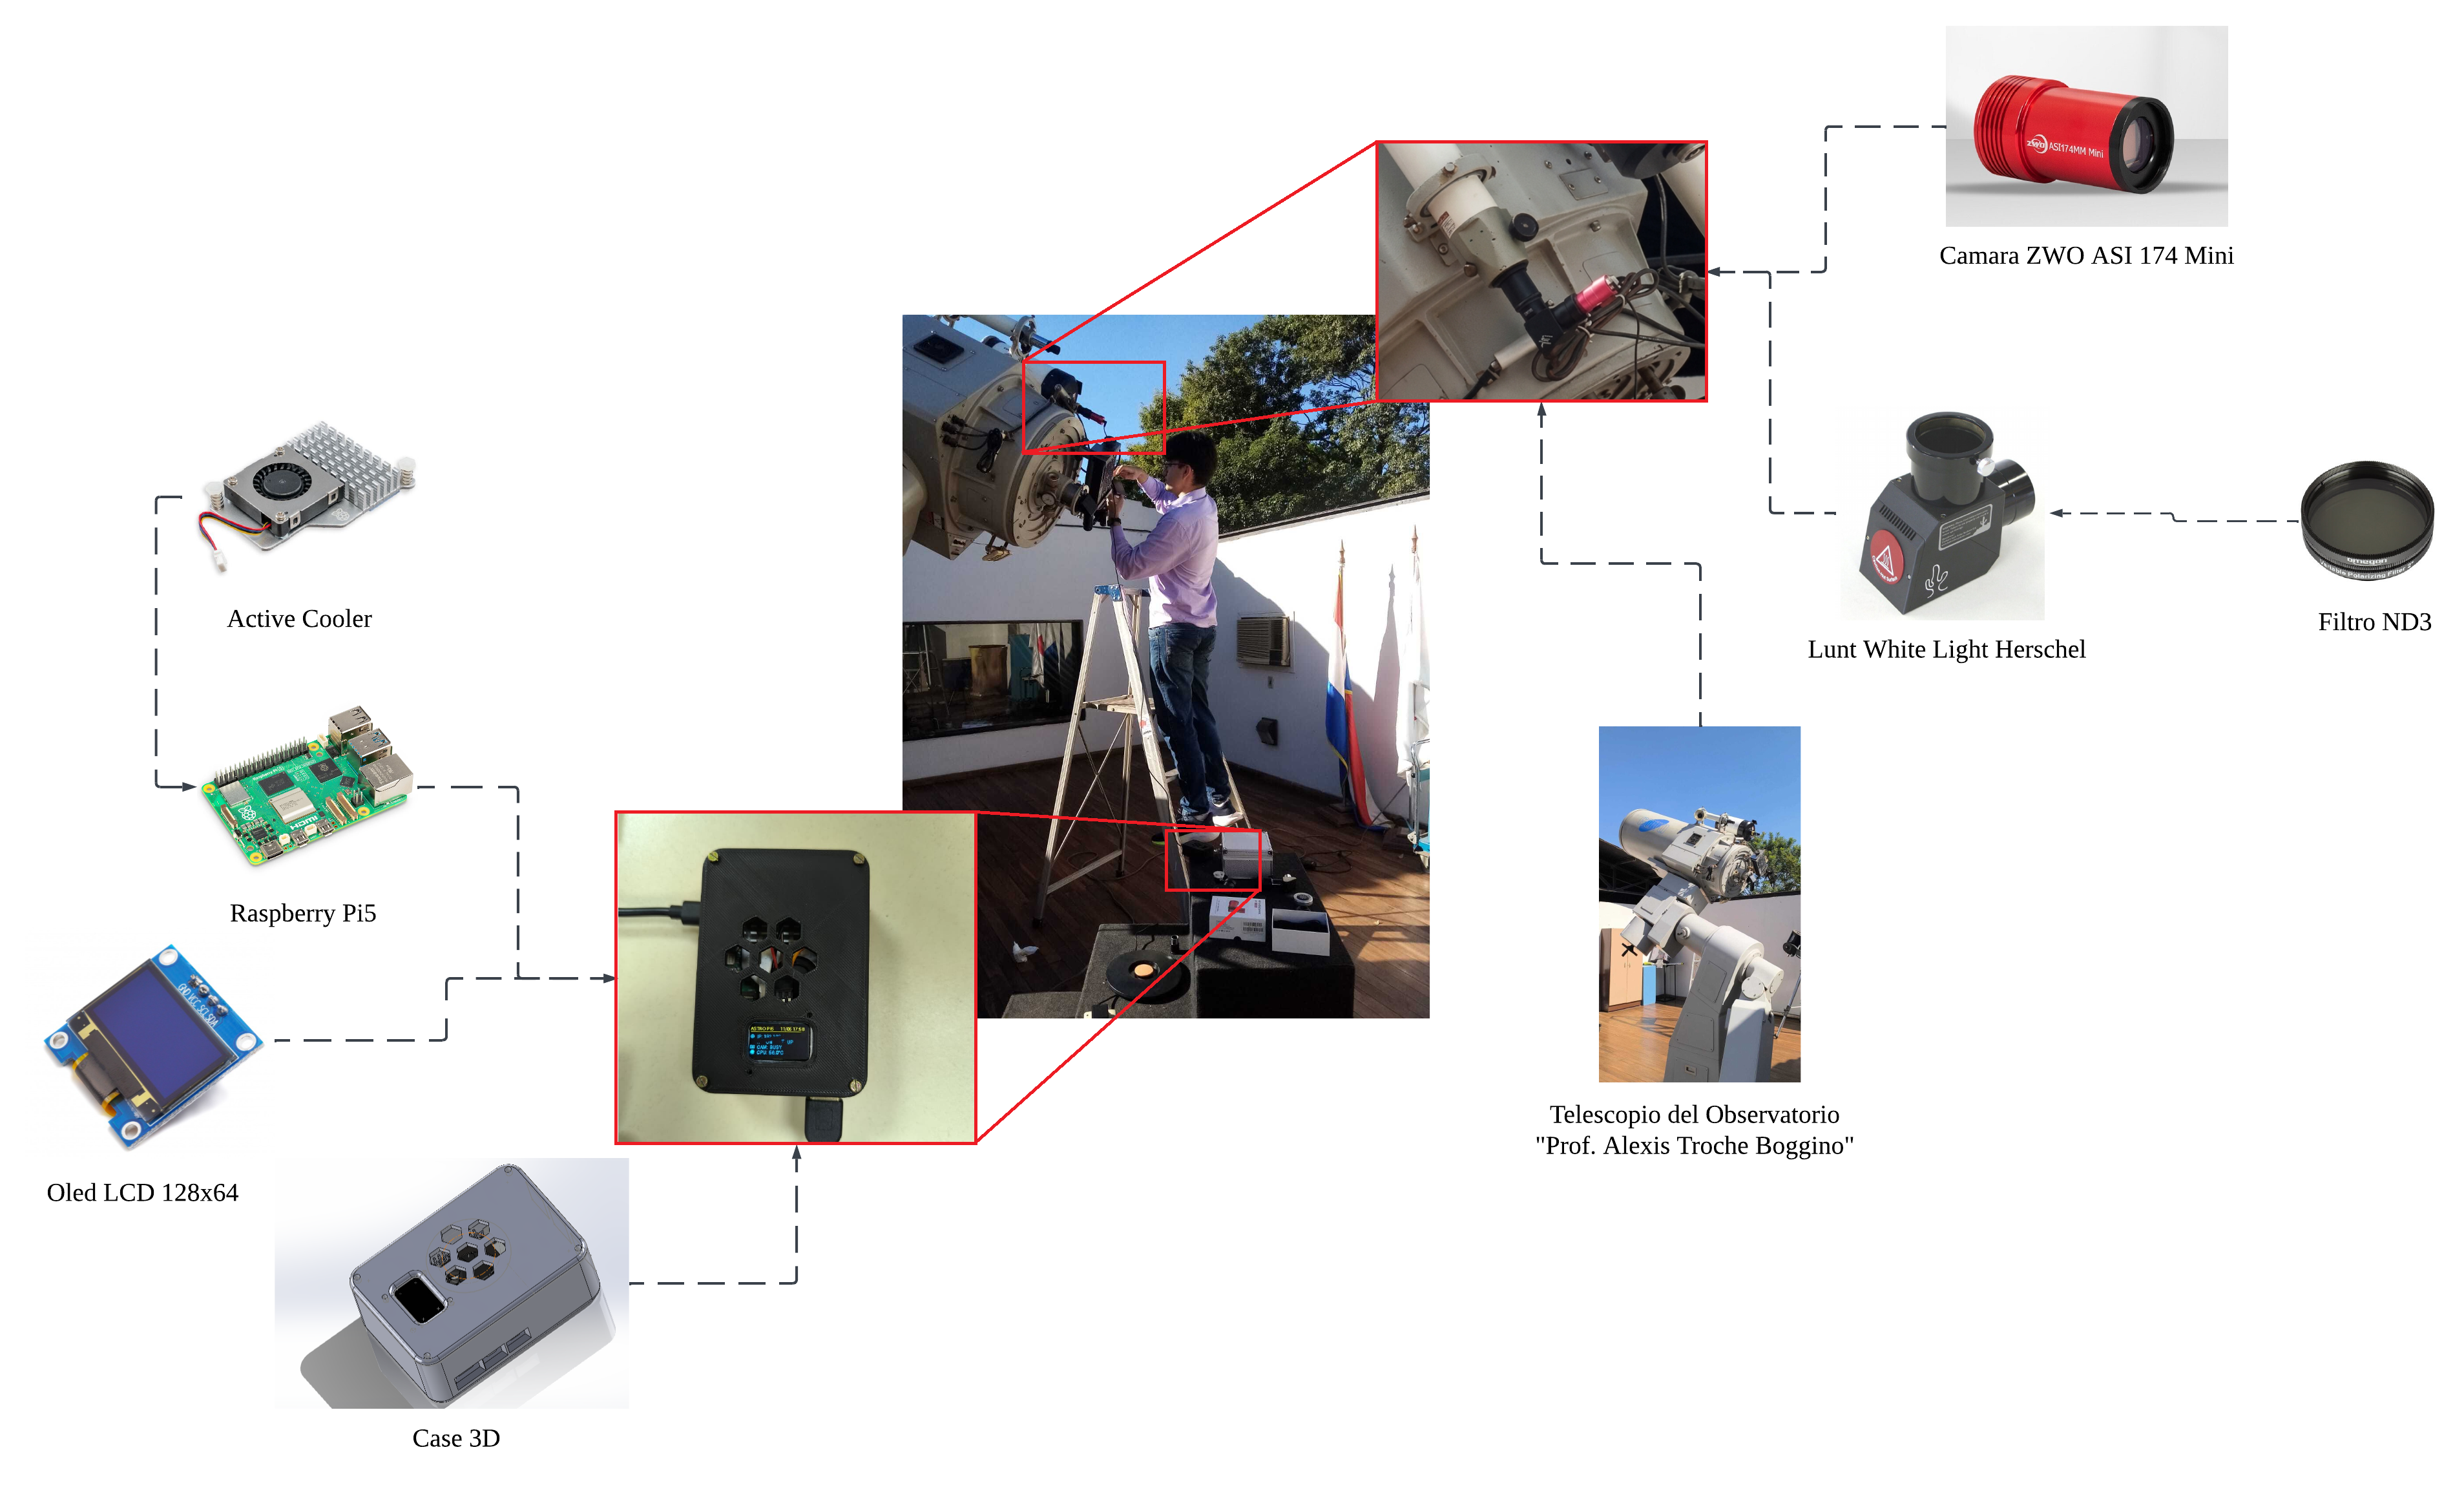
\includegraphics[width=0.88\textwidth]{hw/hw_diagram.png}
    \caption{Componentes del flujo de adquisición, procesamiento local y publicación de datos.}
    \label{fig:hardware-diagrama}
\end{figure*}
El módulo de observación emplea una cámara monocromática ZWO ASI174MM Mini, un sistema de atenuación óptica con cuña de Herschel y un telescopio refractor para capturar imágenes solares en luz blanca. La selección de la cámara priorizó sensor monocromático, obturador global, píxel de 5.86 $\mu$m, área efectiva amplia y compatibilidad mecánica con trenes ópticos compactos; estas condiciones favorecen nitidez espacial, estabilidad temporal y reducción de artefactos por \textit{seeing} variable. La cuña de Herschel se adoptó como solución de atenuación para refractores, preservando contraste en umbra y penumbra y evitando saturación del sensor. La unidad de procesamiento se implementó sobre Raspberry Pi 5 con refrigeración activa, almacenamiento local, pantalla de estado y conectividad de red, lo que permite ejecutar captura, preprocesamiento y sincronización cerca del punto de observación \citep{zwoASI174Manual2025,zwoASILinuxManual,luntWhiteLightWedges2026,nmcliHotspot2026}.

\subsection{Cadena de datos e inteligencia artificial}
\begin{figure*}[t]
    \centering
    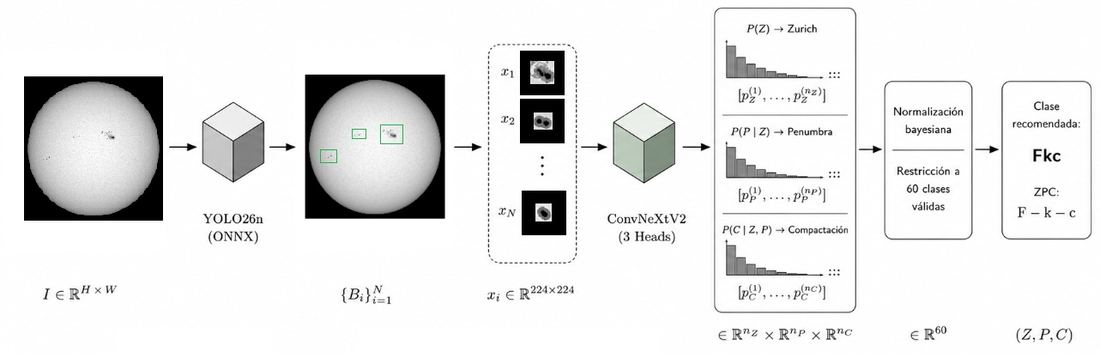
\includegraphics[width=0.96\textwidth]{sys/img_pipe.jpg}
    \caption{Cadena de procesamiento de imágenes solares.}
    \label{fig:pipeline}
\end{figure*}
\begin{figure*}[t]
    \centering
    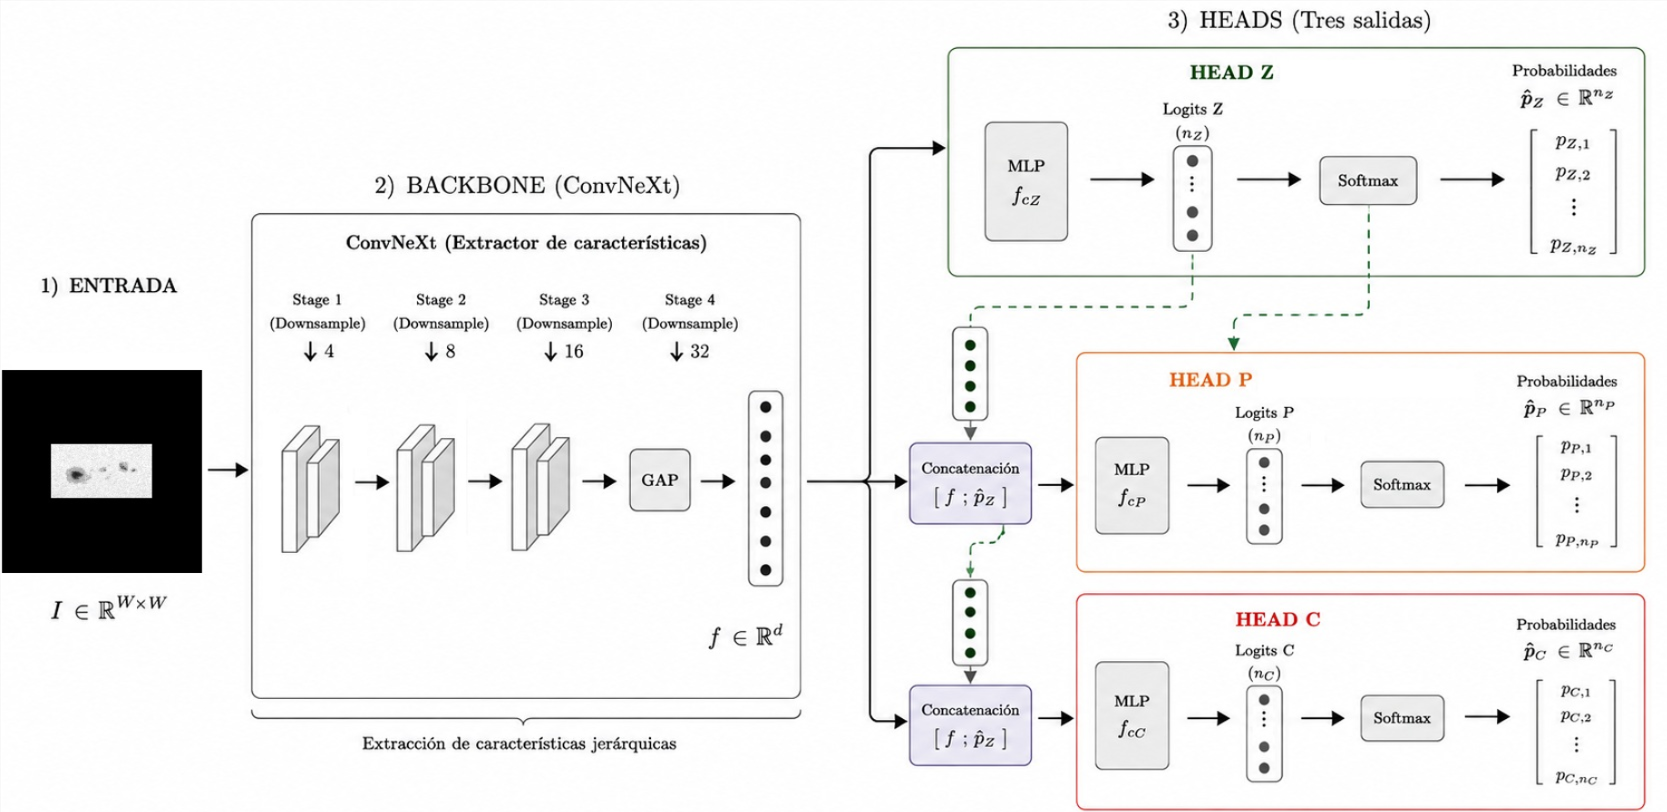
\includegraphics[width=0.96\textwidth]{ml/convnext_arch.png}
    \caption{Arquitectura jerárquica ConvNeXtV2a para componentes Zurich--McIntosh.}
    \label{fig:convnext-arch}
\end{figure*}

La base de datos fue construida a partir de imágenes SDO/HMI, reportes NOAA SRS y registros propios. El acoplamiento SDO--NOAA permite usar la estabilidad temporal y disponibilidad pública de HMI para generar pares imagen--reporte útiles para entrenamiento supervisado, mientras que las capturas locales sirven para validar el dominio final de aplicación. La primera etapa de IA se formula como un problema de detección de objetos: YOLO26n estima cajas delimitadoras $b_i=(x_i,y_i,w_i,h_i)$ para cada grupo solar visible en una imagen de disco completo. La segunda etapa recibe recortes normalizados y estima la etiqueta Zurich--McIntosh. En lugar de aprender una clase plana $ZPC$, el sistema emplea un clasificador jerárquico basado en ConvNeXtV2a con salidas separadas para $Z$, $P$ y $C$ \citep{scherrer2012hmi,bobra2014sharp,noaaSRS,ultralyticsYOLO26,woo2023convnextv2}.

Para un recorte $x\in\mathbb{R}^{224\times224}$, el backbone ConvNeXtV2 produce mapas de características que se resumen mediante agrupamiento promedio global en un vector
\begin{equation}
\mathbf{f}=\operatorname{GAP}(\operatorname{ConvNeXtV2}(x)), \qquad \mathbf{f}\in\mathbb{R}^{d}.
\end{equation}
La primera salida estima la distribución del carácter Zurich,
\begin{equation}
\hat{\mathbf{p}}_Z=\operatorname{softmax}(g_Z(\mathbf{f})), \qquad \hat{\mathbf{p}}_Z\in\mathbb{R}^{n_Z}.
\end{equation}
Luego, las salidas penumbral y de compactación incorporan la dependencia con $Z$ usando la concatenación del vector visual y la distribución Zurich:
\begin{equation}
\begin{aligned}
\hat{\mathbf{p}}_P&=\operatorname{softmax}(g_P([\mathbf{f};\hat{\mathbf{p}}_Z])),\\
\hat{\mathbf{p}}_C&=\operatorname{softmax}(g_C([\mathbf{f};\hat{\mathbf{p}}_Z])).
\end{aligned}
\end{equation}
Por tanto, el clasificador se expresa como
\begin{equation}
f_\theta(x)=\left(\hat{\mathbf{p}}_Z,\hat{\mathbf{p}}_P,\hat{\mathbf{p}}_C\right),
\end{equation}
donde cada término es una distribución probabilística sobre una componente de la taxonomía. La probabilidad conjunta ideal se expresa como
\begin{equation}
\begin{aligned}
P(Z,P,C\mid x)&=P(Z\mid x)P(P\mid Z,x)\\
&\quad \times P(C\mid Z,P,x).
\end{aligned}
\end{equation}
Como implementación operativa se usa una base factorizada,
\begin{equation}
P_{\mathrm{base}}(Z,P,C\mid x)=P(Z\mid x)P(P\mid x)P(C\mid x),
\end{equation}
y se aplica una máscara binaria $M_{ZPC}$ para anular combinaciones no admisibles. La distribución recomendada queda normalizada como
\begin{equation}
\begin{aligned}
P_{\mathrm{rec}}(Z,P,C\mid x)&=
P_{\mathrm{base}}(Z,P,C\mid x)M_{ZPC}\\
&\quad \Big/ \sum_{z,p,c}P_{\mathrm{base}}(z,p,c\mid x)M_{zpc}.
\end{aligned}
\end{equation}
La clase final se obtiene con $(Z^\ast,P^\ast,C^\ast)=\arg\max_{Z,P,C}P_{\mathrm{rec}}(Z,P,C\mid x)$, manteniendo interpretabilidad y consistencia taxonómica \citep{mcintosh1990classification,bornmann1994flarerates,cui2019classbalanced,sayez2023sunscc}.

\subsection{Modelos predictivos y plataforma web}
El análisis predictivo combina una representación escalar del número de manchas solares y una representación espacio-temporal del diagrama de Spörer. Para los modelos predictivos, el número de manchas solares suavizado se estima con PVL--Kalman. La etapa de actualización queda dada por
\begin{equation}
K_k=P_k^{-}(P_k^{-}+R_k)^{-1}, \qquad
\widehat{s}_k=\widehat{s}_k^{-}+K_k(z_k-\widehat{s}_k^{-}),
\end{equation}
donde $z_k$ es la observación mensual y $\widehat{s}_k$ la estimación corregida. Este bloque resume la amplitud temporal del ciclo solar mediante una serie escalar \citep{kalman1960newapproach,podladchikova2012kalman}.

El modelo DMD complementa esa salida escalar con una reconstrucción de la distribución latitudinal de actividad. Cada observación mensual se transforma en un vector de conteos latitudinales. Sea $N_{\mathrm{spots}}(t)$ el número total de manchas en el instante $t$ y $\theta_i(t)$ la latitud heliográfica de la $i$-ésima mancha; el dominio se restringe a
\begin{equation}
\theta\in[-50^{\circ},50^{\circ}], \qquad \Delta\theta=4^{\circ}, \qquad M=25.
\end{equation}
El $j$-ésimo contenedor se define como $\mathcal{B}_j=[\theta_j,\theta_{j+1})$ y su conteo como
\begin{align}
V_j(t)&=\sum_{i=1}^{N_{\mathrm{spots}}(t)}\Psi_{j,i}(t),\\
\Psi_{j,i}(t)&=
\begin{cases}
1, & \theta_i(t)\in\mathcal{B}_j,\\
0, & \theta_i(t)\notin\mathcal{B}_j.
\end{cases}
\end{align}
de modo que $\Psi_{j,i}(t)$ actúa como función indicadora de pertenencia de la mancha $i$ al contenedor latitudinal $j$. Con ello, el estado latitudinal mensual queda dado por
\begin{equation}
\mathbf{x}_t=\begin{bmatrix}V_1(t)&V_2(t)&\cdots&V_M(t)\end{bmatrix}^{T}\in\mathbb{R}^{M},
\end{equation}
y la secuencia histórica se organiza como matriz de instantáneas:
\begin{equation}
\mathbf{X}=\begin{bmatrix}\mathbf{x}_1&\mathbf{x}_2&\cdots&\mathbf{x}_N\end{bmatrix}\in\mathbb{R}^{M\times N}.
\end{equation}

La Descomposición en Modos Dinámicos aproxima la evolución mediante un operador lineal efectivo $\mathbf{A}$, de modo que
\begin{equation}
\mathbf{x}_{k+1}\approx\mathbf{A}\mathbf{x}_{k}.
\end{equation}
A partir de $\mathbf{X}$ se construyen matrices desplazadas de estados consecutivos:
\begin{equation}
\mathbf{X}_1=\begin{bmatrix}\mathbf{x}_1&\cdots&\mathbf{x}_{N-1}\end{bmatrix},\quad
\mathbf{X}_2=\begin{bmatrix}\mathbf{x}_2&\cdots&\mathbf{x}_{N}\end{bmatrix}.
\end{equation}
El operador se estima con una SVD truncada de rango $r=10$,
\begin{equation}
\mathbf{X}_1\approx\mathbf{U}_r\boldsymbol{\Sigma}_r\mathbf{V}_r^{H},
\end{equation}
y se reconstruye como
\begin{equation}
\mathbf{A}\approx\mathbf{X}_2\mathbf{V}_r\boldsymbol{\Sigma}_r^{-1}\mathbf{U}_r^{H}.
\end{equation}
La proyección futura se calcula iterativamente mediante
\begin{equation}
\widehat{\mathbf{x}}_{k+1}=\mathbf{A}\widehat{\mathbf{x}}_k, \qquad k>N.
\end{equation}
Finalmente, el índice global derivado de DMD se obtiene integrando la distribución latitudinal predicha:
\begin{equation}
\widehat{\mathbf{x}}_t=\begin{bmatrix}\widehat{V}_1(t)&\widehat{V}_2(t)&\cdots&\widehat{V}_M(t)\end{bmatrix}^{T},
\end{equation}
\begin{align}
\mathrm{SSN}_{\mathrm{DMD}}(t)&=\kappa\sum_{j=1}^{M}\widehat{V}_j(t),\\
\kappa&=\frac{\sum_{t=1}^{N}\mathrm{SSN}_{\mathrm{obs}}(t)}
{\sum_{t=1}^{N}\sum_{j=1}^{M}\widehat{V}_j(t)}.
\end{align}
Estas ecuaciones permiten pasar de una representación latitudinal física a una magnitud comparable con el SSN histórico, sin perder la lectura espacio-temporal del diagrama de Spörer. La plataforma web permite cargar imágenes, consultar Supabase y ejecutar modelos ONNX en navegador mediante WebAssembly. Esta decisión reduce la dependencia de un servidor central de inferencia, facilita actualizaciones de modelos livianos y mantiene parte del procesamiento cerca del usuario, aspecto relevante para escenarios con conectividad intermitente \citep{schmid2010dmd,kutz2016dmd,hathaway2015solarcycle,woo2023convnextv2,ultralyticsYOLO26,camporeale2019ml}.

\section{Resultados y discusión}
\subsection{Validación de clasificación}
\begin{figure}[H]
    \centering
    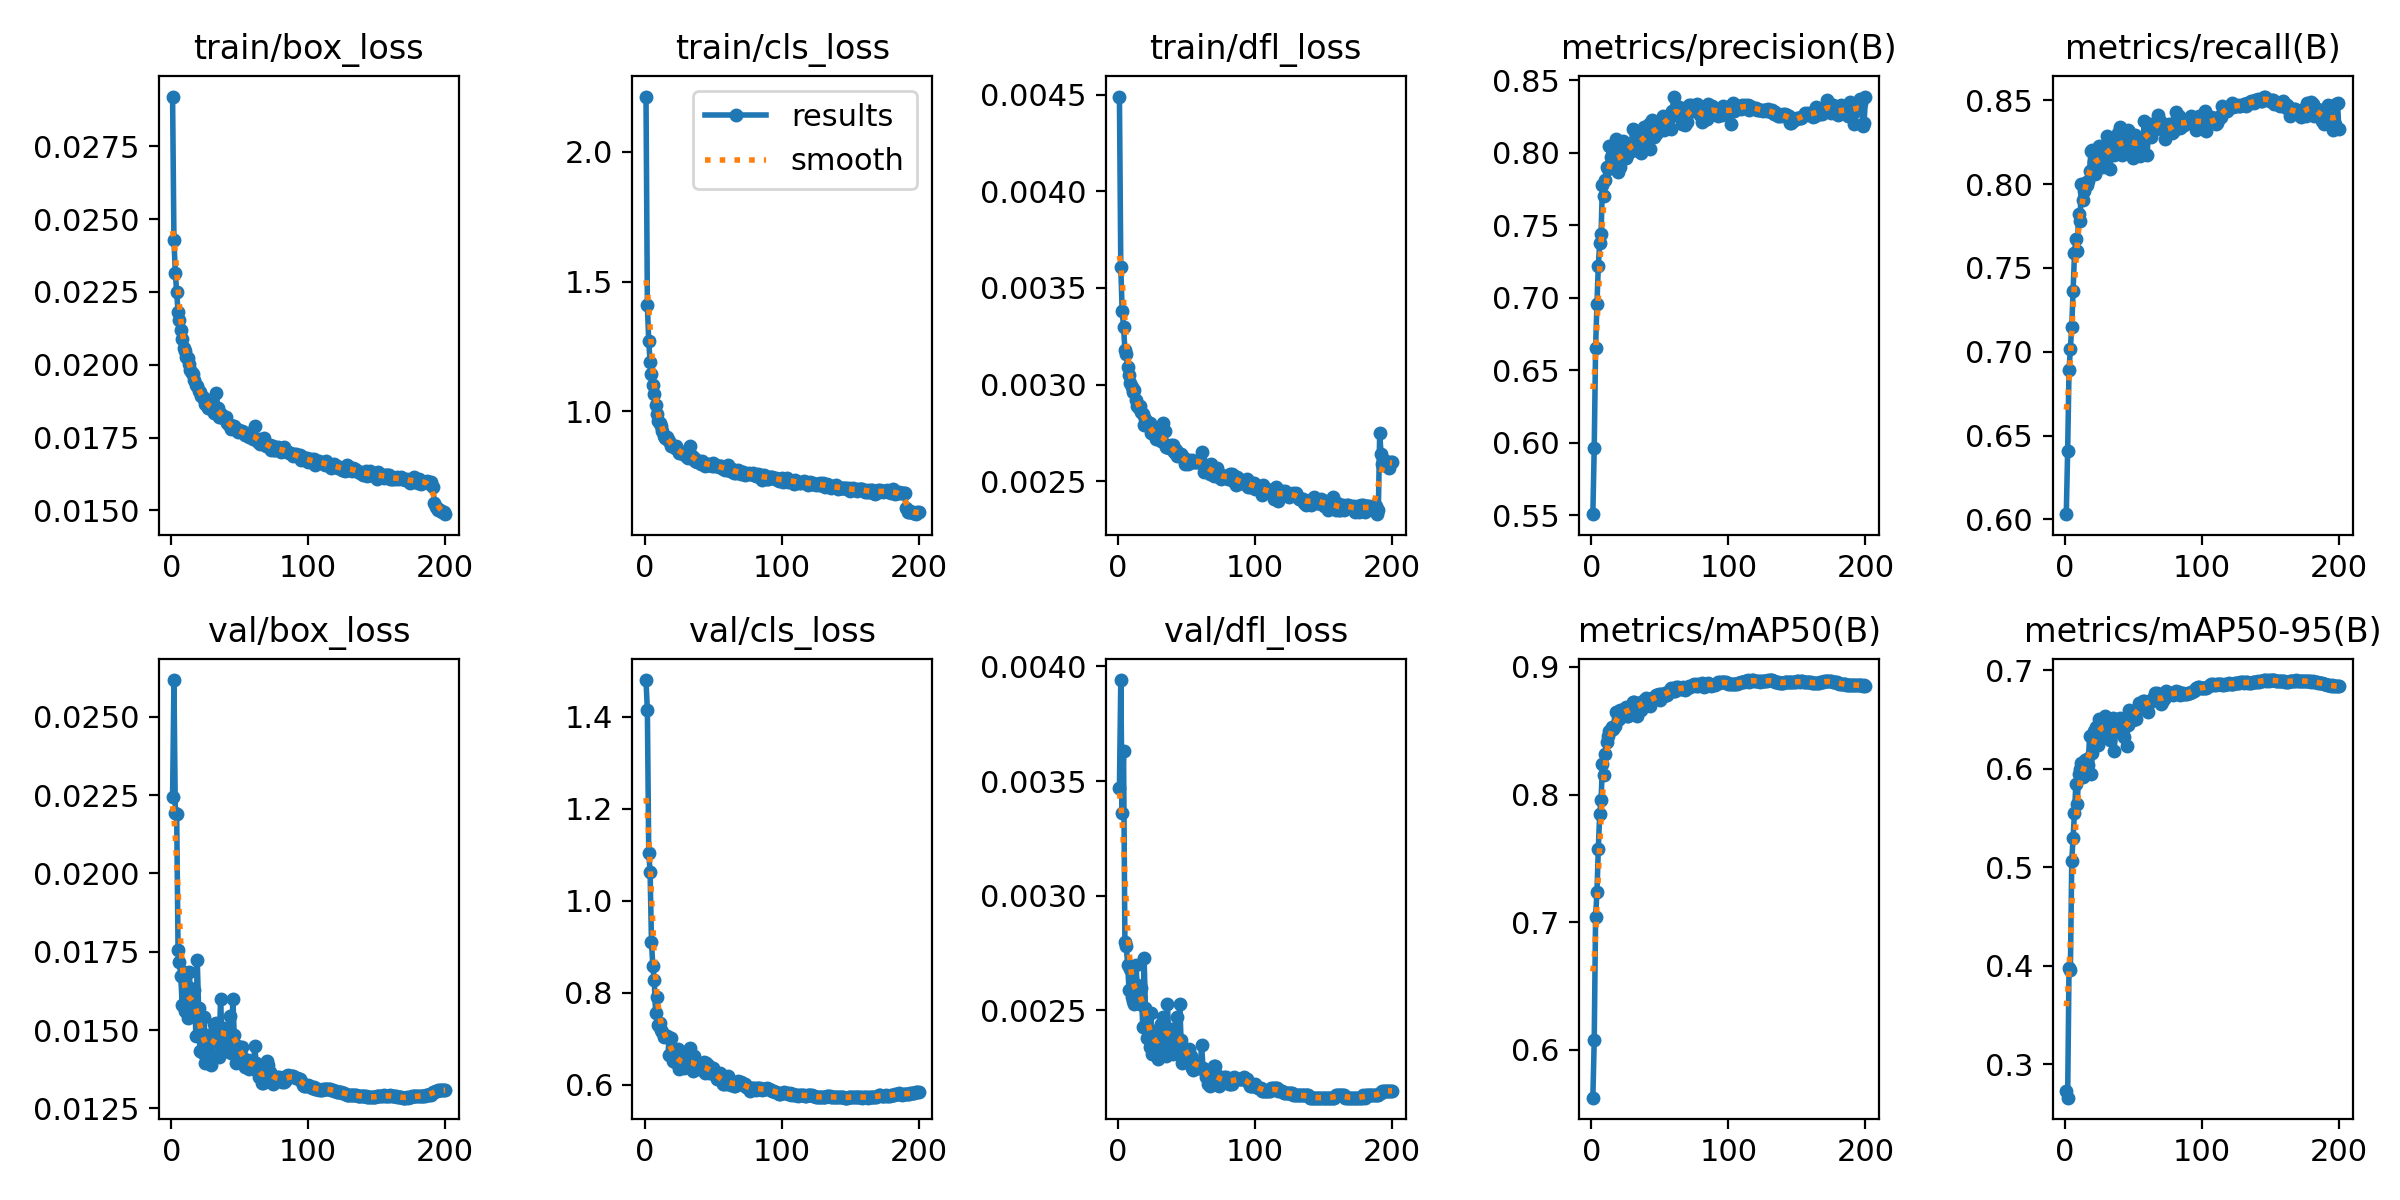
\includegraphics[width=0.92\linewidth]{ml/yolo_results.png}
    \caption{Resultados del agrupamiento de regiones activas mediante YOLO26n.}
    \label{fig:yolo-resultados}
\end{figure}
\begin{figure}[H]
    \centering
    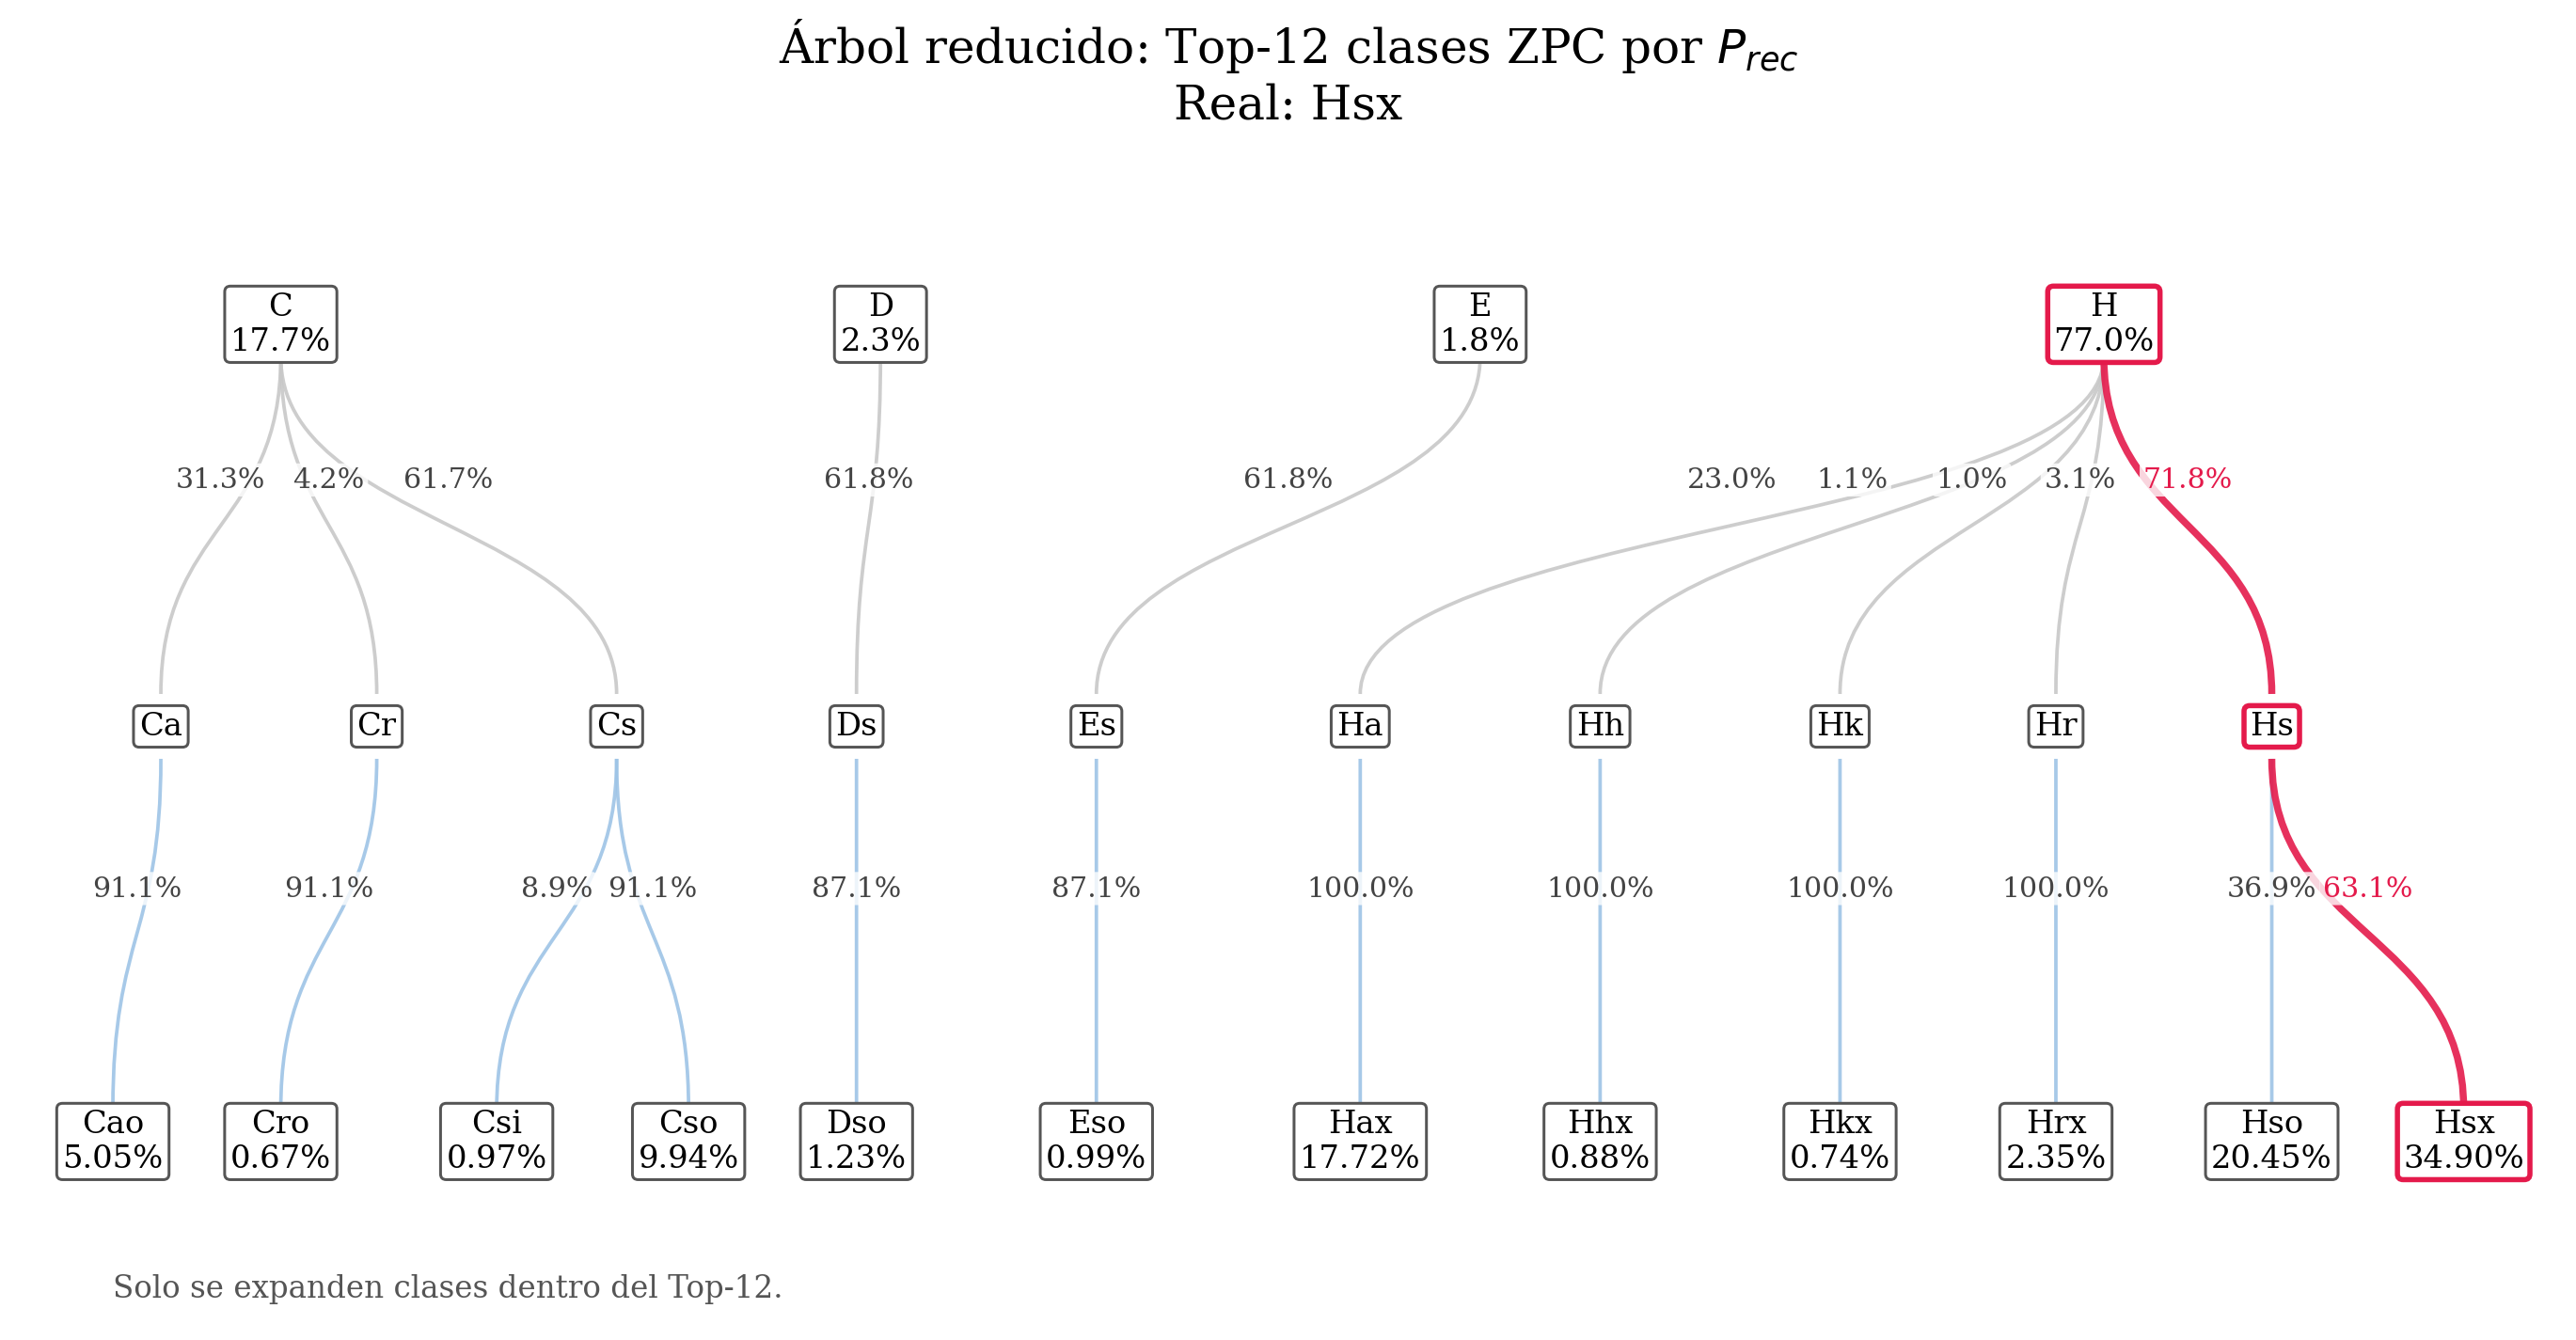
\includegraphics[width=0.92\linewidth]{ml/top12_tree.png}
    \caption{Árbol bayesiano de probabilidades para recomendación jerárquica Zurich--McIntosh.}
    \label{fig:top12-tree}
\end{figure}

Los resultados experimentales confirman que la separación entre detección y clasificación es adecuada: YOLO26n localiza grupos solares y genera recortes para la etapa morfológica, mientras que ConvNeXtV2a conserva salidas independientes para $Z$, $P$ y $C$. Esta división reduce la complejidad de cada tarea y se alinea con la práctica observacional: primero se identifica la unidad física relevante, el grupo solar, y luego se describe su morfología. Además, evita compactar artificialmente clases raras y ofrece probabilidades interpretables en lugar de una única etiqueta opaca \citep{sayez2023sunscc,deng2025mcintosh,palladino2022sunspot}.
\begin{table}[htbp]
\centering
\caption{Métricas resumidas del clasificador jerárquico Zurich--McIntosh.}
\footnotesize
\renewcommand{\arraystretch}{0.95}
\begin{tabular}{lccc}
\toprule
\textbf{Salida} & \textbf{Precisión pond.} & \textbf{Recall pond.} & \textbf{F1 pond.} \\
\midrule
Z & 0.68 & 0.63 & 0.65 \\
P & 0.66 & 0.61 & 0.63 \\
C & 0.74 & 0.69 & 0.71 \\
\bottomrule
\end{tabular}
\end{table}

Los valores muestran desempeño consistente para clases frecuentes, aunque el desbalance de clases y la ambigüedad morfológica afectan clases raras o visualmente cercanas. Estas limitaciones son esperables en la taxonomía Zurich--McIntosh, cuya distribución de combinaciones presenta cola larga y fronteras observacionales no siempre nítidas. En este contexto, la máscara de combinaciones válidas y el árbol de recomendaciones no eliminan el ruido de etiqueta, pero restringen el espacio de salida y convierten la predicción en una herramienta de asistencia revisable por el observador.

\subsection{Validación predictiva y operacional}
\begin{figure}[H]
    \centering
    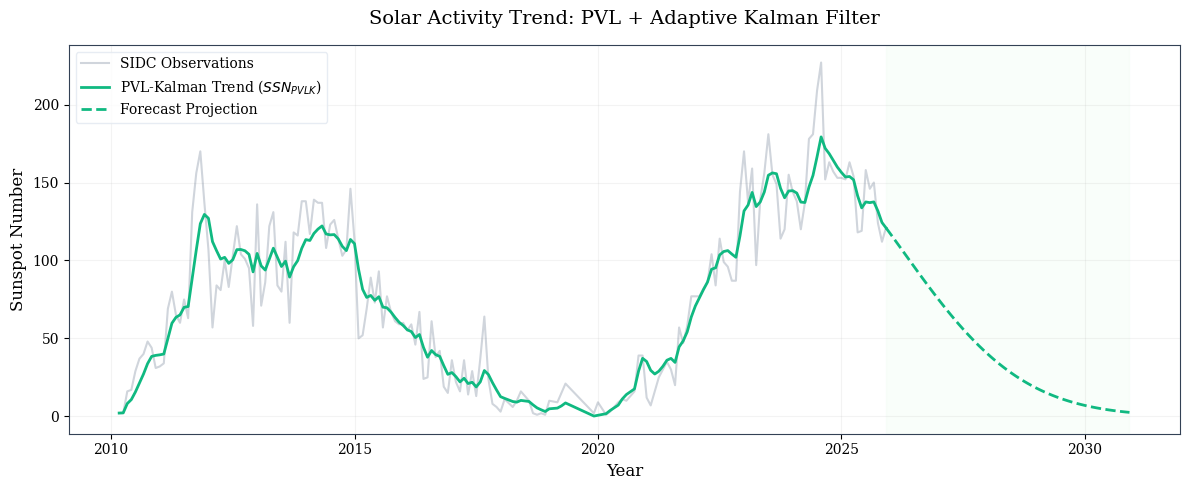
\includegraphics[width=0.92\linewidth]{pred/kalman.png}
    \caption{Ajuste y predicción del número de manchas solares mediante PVL--Kalman.}
    \label{fig:pvl-kalman}
\end{figure}
\begin{figure}[H]
    \centering
    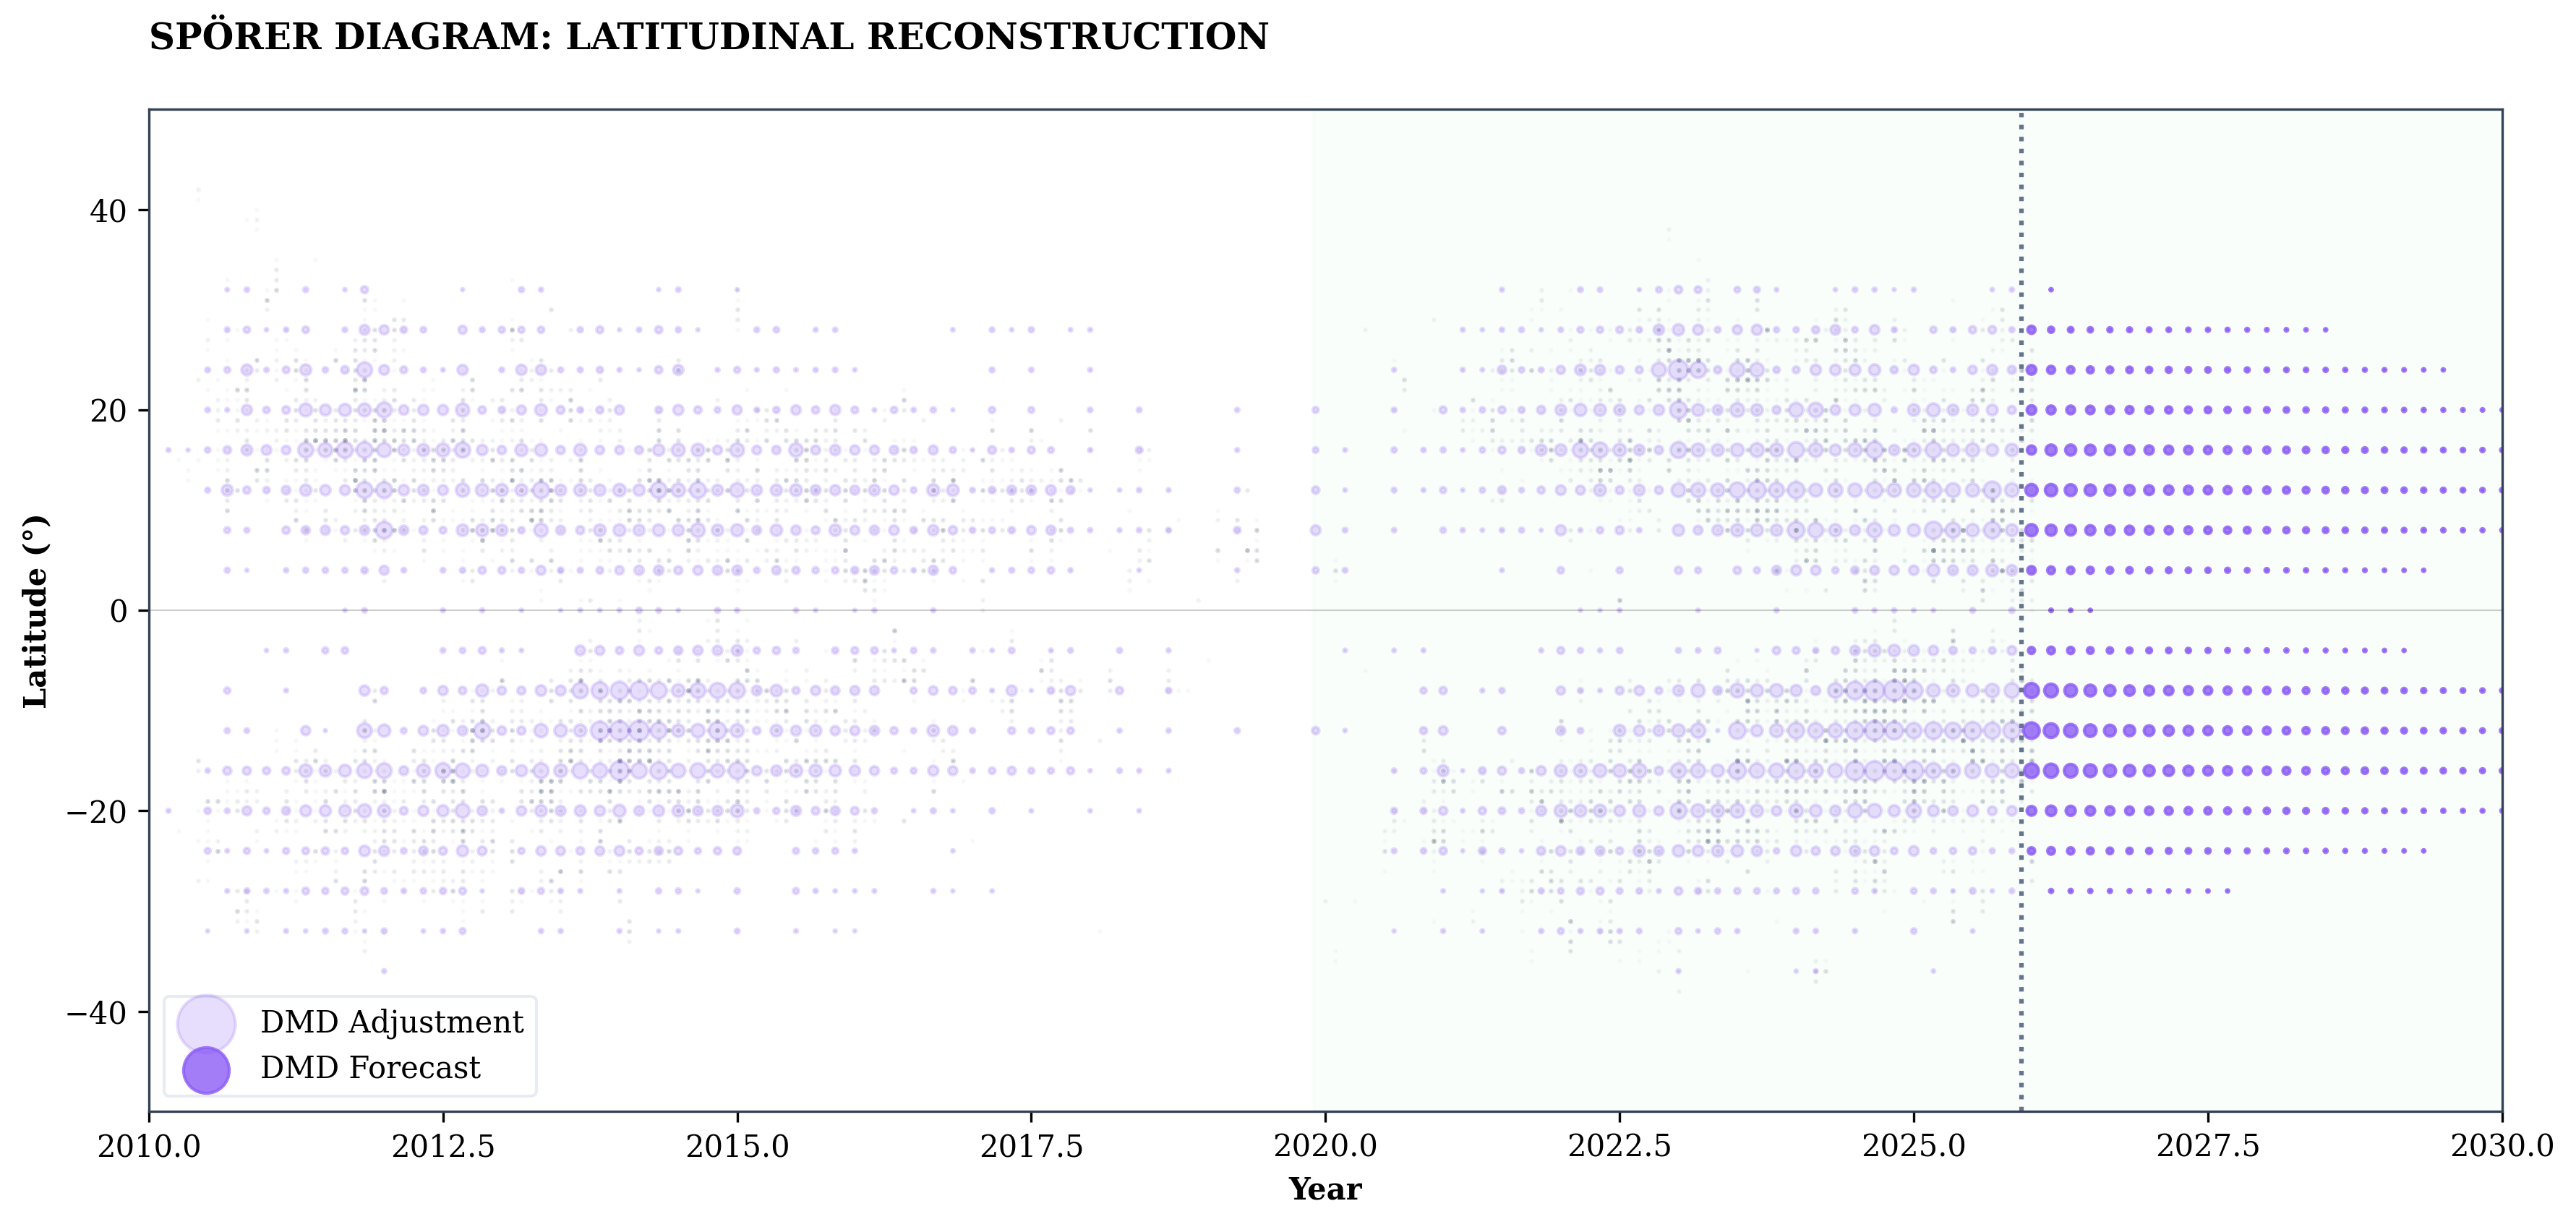
\includegraphics[width=0.92\linewidth]{pred/sporer.png}
    \caption{Reconstrucción y predicción de la migración latitudinal mediante DMD.}
    \label{fig:sporer-dmd}
\end{figure}

Para el SSN se emplearon MAE, RMSE, MAPE y $R^2$; para la reconstrucción latitudinal se emplearon el error relativo de Frobenius $E_F$, la correlación espacio-temporal $\rho_{ST}$ y el error medio de latitud central $\mathrm{MLCE}$. Estas métricas distinguen la precisión escalar de la fidelidad espacial de la migración tipo Spörer.
\begin{table}[htbp]
\centering
\caption{Métricas principales de validación predictiva.}
\footnotesize
\begin{tabular}{lcc}
\toprule
\textbf{Métrica} & \textbf{$\mathrm{SSN}_{\mathrm{PVLK}}$} & \textbf{$\mathrm{SSN}_{\mathrm{DMD}}$} \\
\midrule
$\mathrm{MAE}$ & 15.31 & 15.22 \\
$\mathrm{RMSE}$ & 22.02 & 20.30 \\
$\mathrm{MAPE}$ & 33.27\% & 32.54\% \\
$R^2$ & 0.8173 & 0.8449 \\
\bottomrule
\end{tabular}
\end{table}

\begin{table}[htbp]
\centering
\caption{Métricas espacio-temporales del modelo DMD--Spörer.}
\footnotesize
\begin{tabular}{lc}
\toprule
\textbf{Indicador} & \textbf{Valor} \\
\midrule
$E_F=\|\mathbf{X}-\widehat{\mathbf{X}}\|_F/\|\mathbf{X}\|_F$ & 0.4087 \\
$\rho_{ST}=\mathrm{corr}(\mathrm{vec}(\mathbf{X}),\mathrm{vec}(\widehat{\mathbf{X}}))$ & 0.9126 \\
$\mathrm{MLCE}=\frac{1}{N}\sum_{k=1}^{N}|\theta_{c,k}-\widehat{\theta}_{c,k}|$ & $1.25^{\circ}$ \\
\bottomrule
\end{tabular}
\end{table}

La captura real del 2026-05-05 verificó adquisición, guardado local, preprocesamiento y sincronización con la base de datos bajo condiciones de operación de campo. Durante los ensayos no se observaron reinicios, cierres del servicio ni reducción térmica perceptible bajo refrigeración activa. La operación representativa incluyó 420 ms para captura individual, 180 ms para guardado local, 1350 ms para preprocesamiento básico, 3800 ms por imagen para sincronización a Supabase, 38\% de CPU media, 72\% de CPU máxima, 3.3 GB de RAM del servicio local y 57 $^{\circ}$C tras 25 minutos \citep{raspberryPi5Docs2026,nmcliHotspot2026}.
\begin{figure}[H]
    \centering
    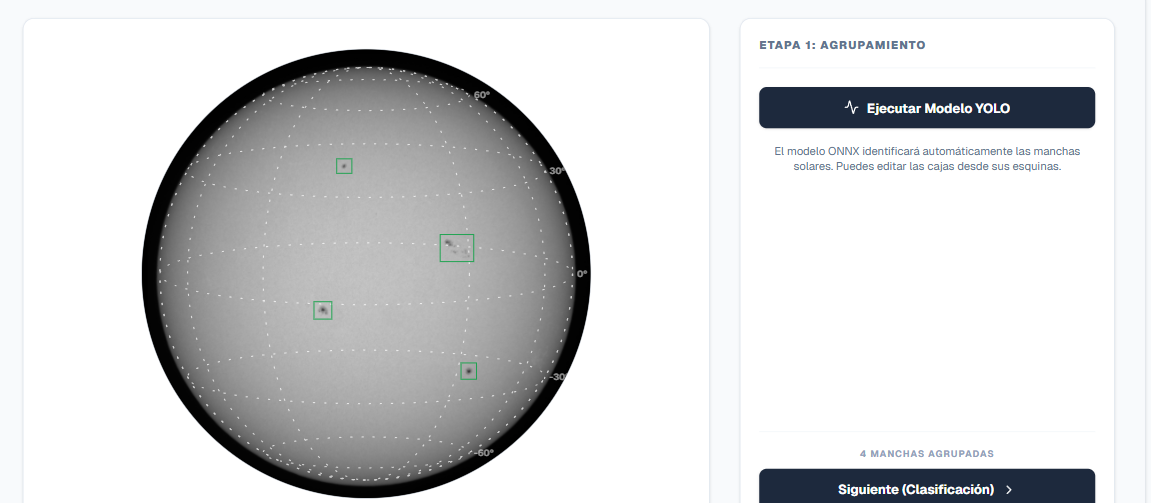
\includegraphics[width=0.9\linewidth]{web/yolo.png}
    \caption{Validación de inferencia local en navegador mediante YOLO26n.}
    \label{fig:web-yolo}
\end{figure}
\begin{figure}[H]
    \centering
    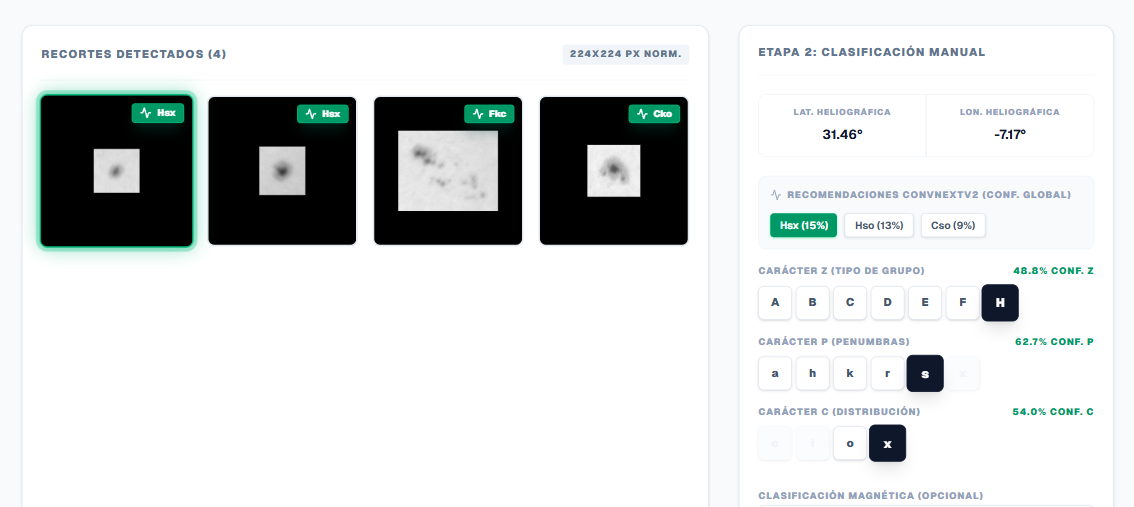
\includegraphics[width=0.9\linewidth]{web/convnext.png}
    \caption{Validación de clasificación morfológica local mediante ConvNeXtV2a.}
    \label{fig:web-convnext}
\end{figure}

\section{Conclusiones}
En este trabajo se presentó un prototipo funcional para observación solar asistida por inteligencia artificial que conecta adquisición, metadatos, inferencia, visualización y análisis temporal. La arquitectura conserva trazabilidad entre imagen original, condiciones instrumentales, recorte, predicción y consulta posterior, condición esencial para aplicaciones científicas y educativas. La principal contribución no radica únicamente en entrenar un detector o un clasificador, sino en integrar esos modelos dentro de una cadena reproducible que transforma una observación solar en un registro auditable y contextualizado.

El enfoque jerárquico resultó apropiado para la taxonomía Zurich--McIntosh, ya que respeta su estructura observacional y evita una clasificación plana de combinaciones. La ejecución local y la conversión de modelos a ONNX refuerzan la portabilidad del sistema, especialmente en observatorios con conectividad limitada. PVL--Kalman y DMD son complementarios: el primero sigue la amplitud global del ciclo solar y el segundo aporta información espacial sobre la migración latitudinal de la actividad.

Como trabajos futuros se propone ampliar campañas de validación bajo diferentes condiciones atmosféricas, mejorar la calibración y el control de exposición, incorporar más datos propios, fortalecer la estimación heliográfica, depurar clases raras de la taxonomía y refinar los modelos predictivos \citep{cesarHeliographic,podladchikova2012kalman,schmid2010dmd}.

\bibliographystyle{apalike}
\bibliography{../fiuna}

\section{Anexo}
El acceso a los recursos digitales del proyecto se organiza mediante códigos QR para facilitar la consulta de la plataforma web y del repositorio de desarrollo.

\begin{figure}[H]
    \centering
    
\includegraphics[width=0.52\linewidth]{qr/web.png}
    \caption{Código QR para acceder a la plataforma web del sistema: \url{https://sunspot-page-app.vercel.app}. \textbf{Fuente:} Elaboración propia.}
    \label{fig:qr-web}
\end{figure}
\begin{figure}[H]
    \centering
    
\includegraphics[width=0.52\linewidth]{qr/repo.png}
    \caption{Código QR para acceder al repositorio del proyecto completo y su documentación: \url{https://github.com/carlobeni/sunspot-page-app/tree/master}. \textbf{Fuente:} Elaboración propia.}
    \label{fig:qr-repo}
\end{figure}

\end{document}
